%Introduction to state charts
\section{State Charts}

Our proposed visual programming language involves using directed state charts with guarded edges. Our languages differs in a few concepts from the usual state charts syntax in order to support features of the hardware. To better understand these differences we will first introduce all the syntax and semantics of a standard UML based state chart.

A State chart is generally defined as a diagram describing the behaviour of a discrete system. Such systems can be either finite state machines, or more complex systems abstracted to resemble a finite state machine. 

%http://en.wikipedia.org/wiki/State_diagram (find different source Taylor atomata paper
Mathematically a state chart can be defined as $M = \lbrace Q, \Sigma, Z, \delta, q_0, F \rbrace$

\begin{itemize}
	\item \textbf{Q:} Set of states.
	\item \textbf{$\Sigma$:} Set of input symbols or actions, these are used when checking guard conditions.
	\item \textbf{Z:} Set of output symbols generated by the system.
	\item \textbf{$\delta$:} Set of state transitions with the mapping $\omega: \Sigma \times Q \rightarrow Z$. These are drawn as arrows and are immediately taken if their guard conditions are true.
	\item \textbf{$q_0$:} Starting state, can be defined as an initial state with no incomming transitions.
	\item \textbf{F:} Accepting states for the system, can also sometimes represent the final state. Drawn as a double outline to the state symbol.
\end{itemize}

A state can be thought of as a set of operating conditions that for example in figure \ref{fig:state_blink_light}
one such state the light is on.

\begin{figure}[htp]
    \centering
    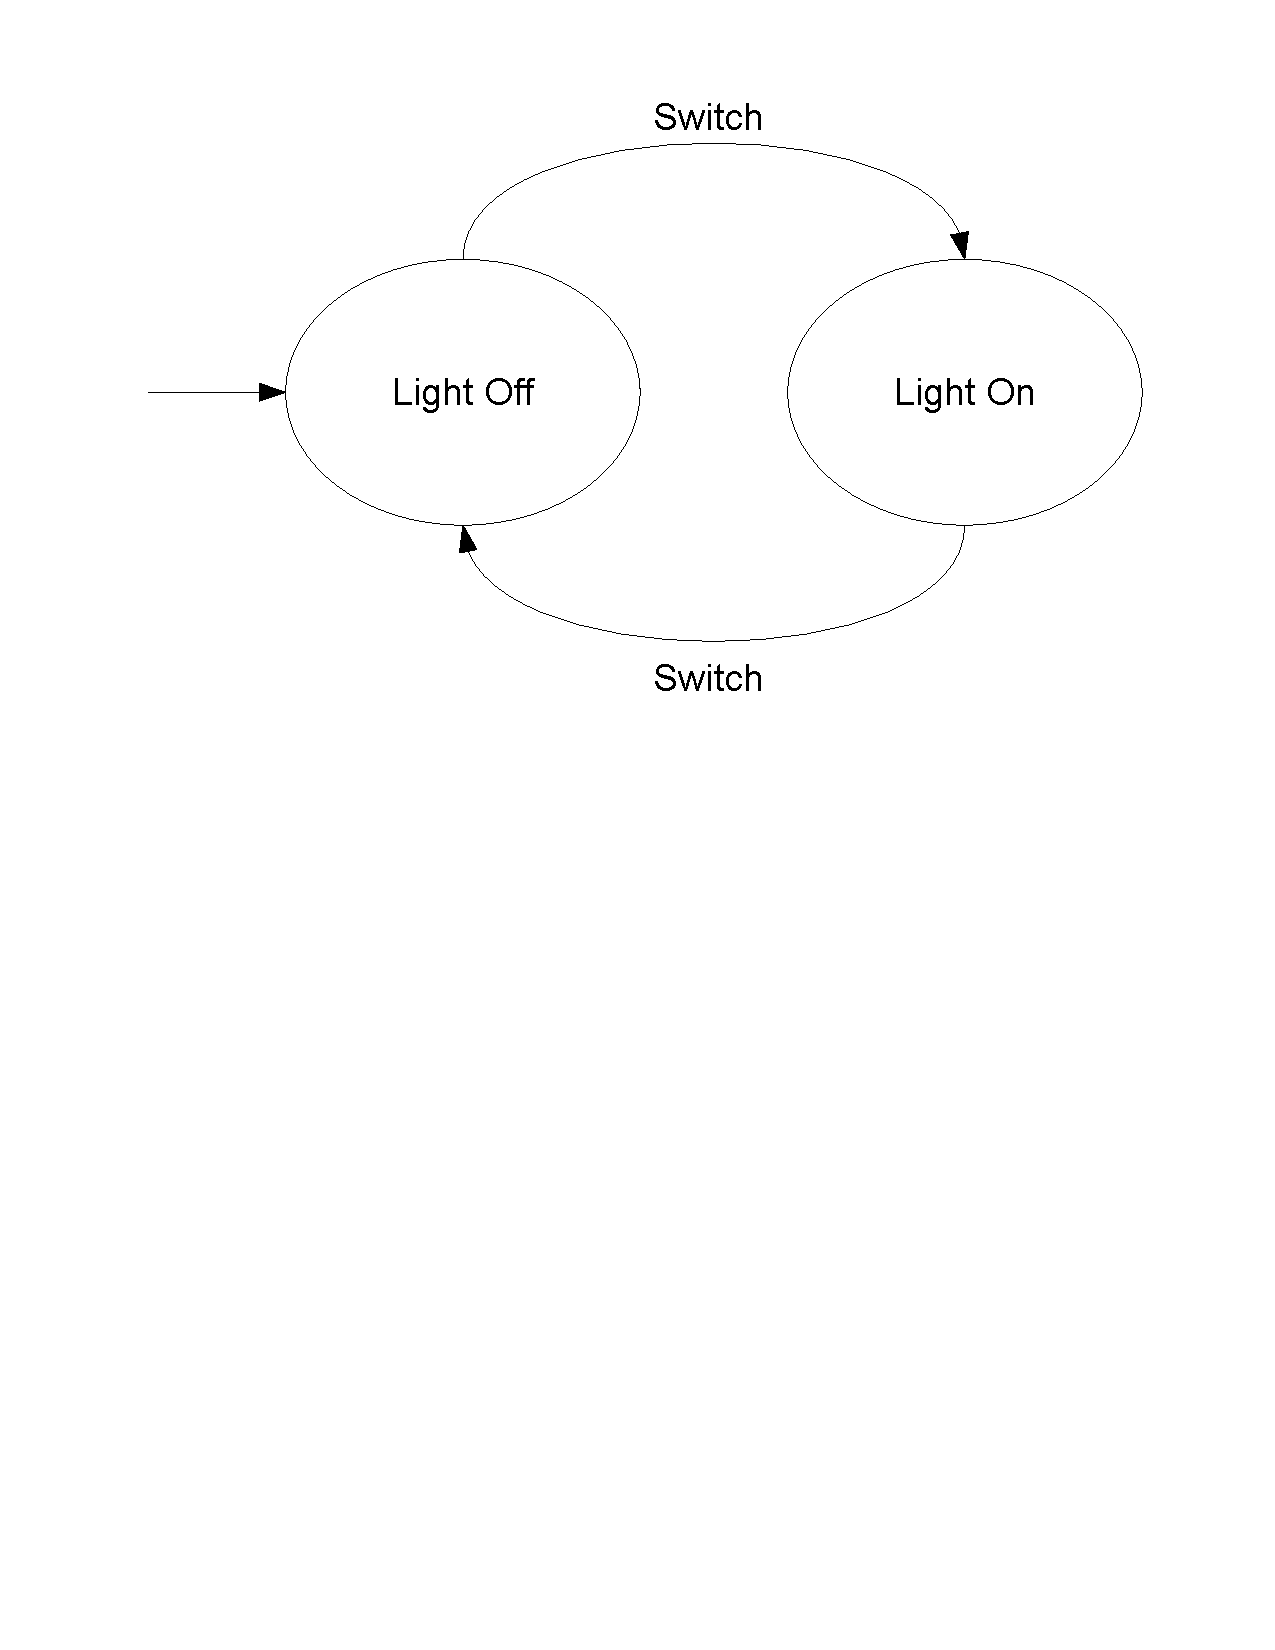
\includegraphics[trim= 10mm 150mm 10mm 10mm, clip ,width=\imgmedium]{./images/state_blink_light.pdf}
    \caption{Simple Toggle Light}
    \label{fig:state_blink_light}
\end{figure}

We observe that transitions must always be connected on the tail end and the tip to a state. In addition if a transition can be taken it must be taken immediately. Transitions may also have a guard condition accociated with them. If a guard condition does not exist then it is assumed the transition can always be taken. In addition to a guard condition each transition may have an output accociated with them. Moore style state machines do not contain outputs on transition edges, Mealy machines do contain an extra output per transition (see: figure \ref{fig:state_moore_mealy}). The output edge on a mealy machine are denoted by a "/" symbol. Although figure \ref{fig:state_moore_mealy} contains outputs for all edges, we can define ourselves a null output or a no change output in order to simulate an edge having no output as well. For purposes of our state chart language we did not require the power of a mealy machine and thus we chose to stay with a simpler moore machine. More details of this decision can be found in the language section \ref{sec:lang:statesemantics} State Chart Semantics.

%diagram for Moore + Mealy state machines
\begin{figure}[htp]
    \centering
    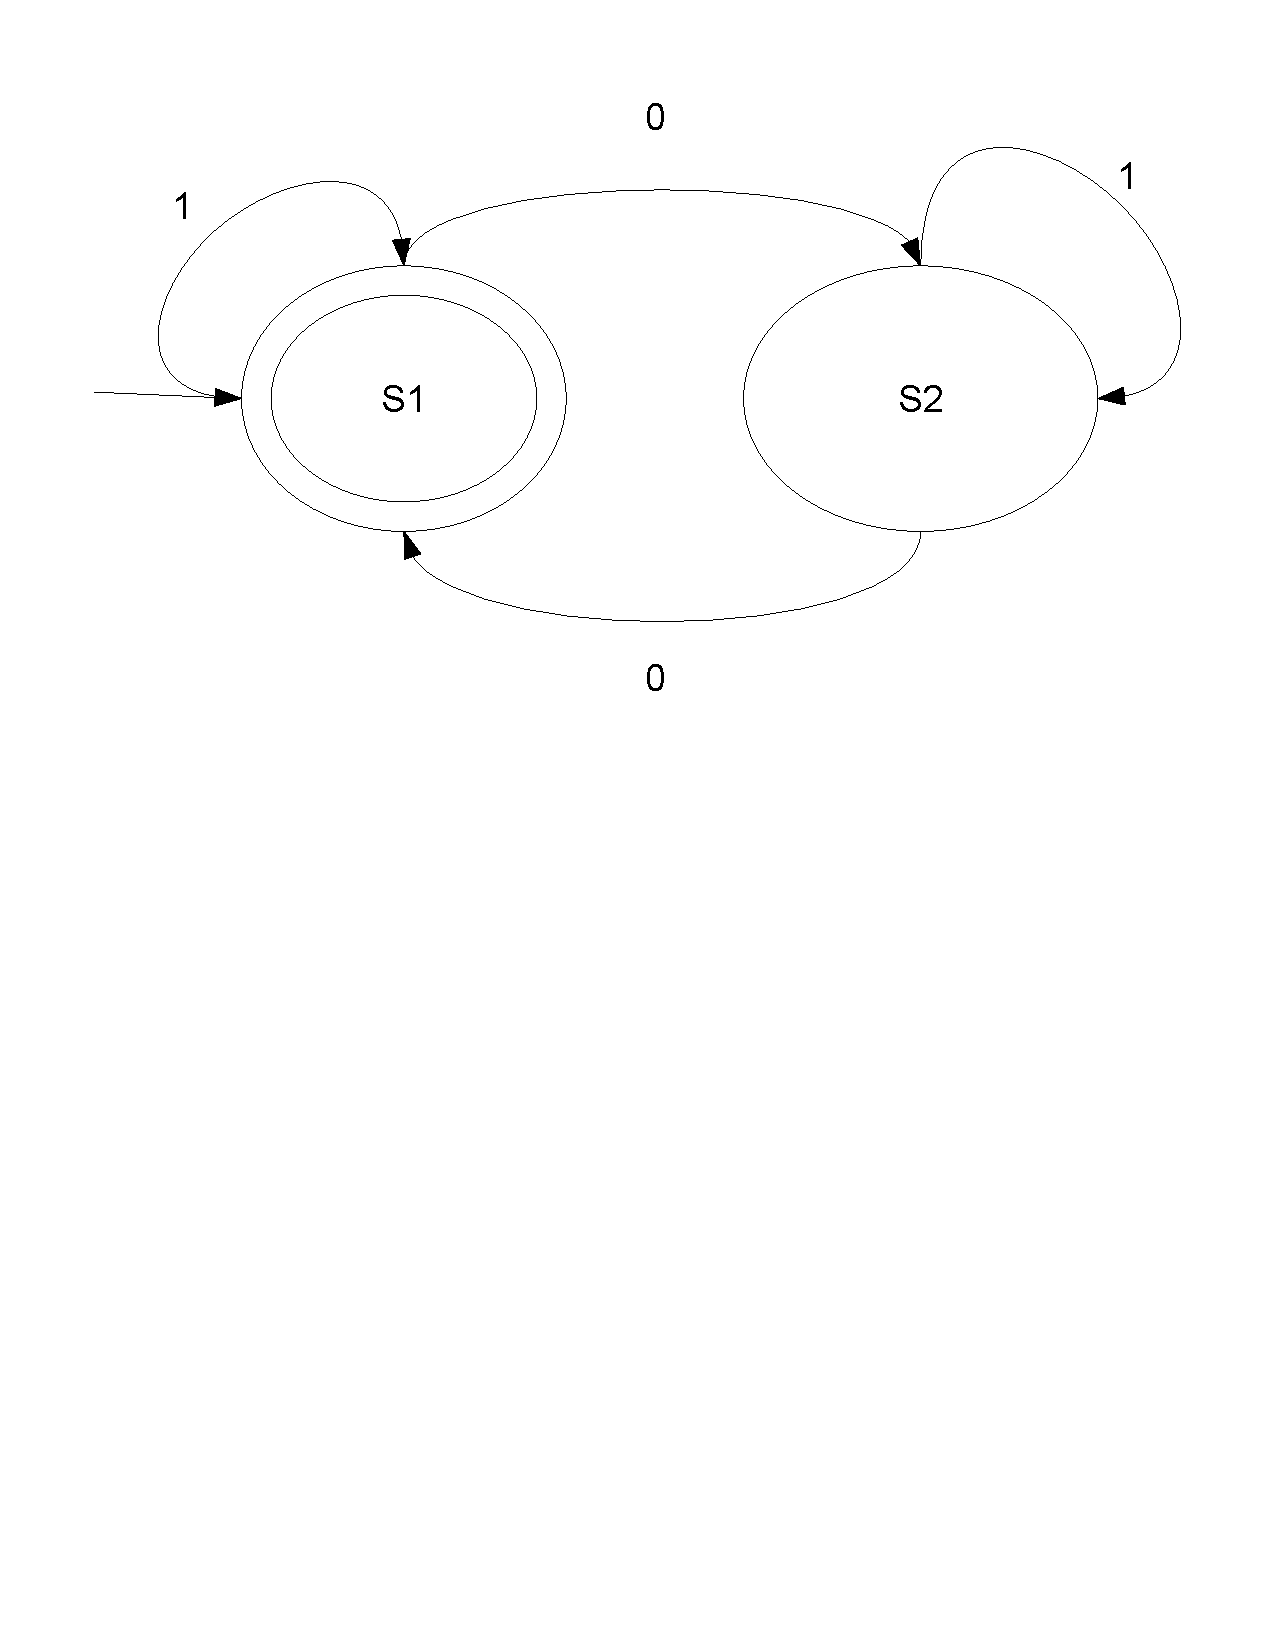
\includegraphics[trim= 15mm 150mm 15mm 10mm, clip ,width=200pt]{./images/state_moore.pdf} 
    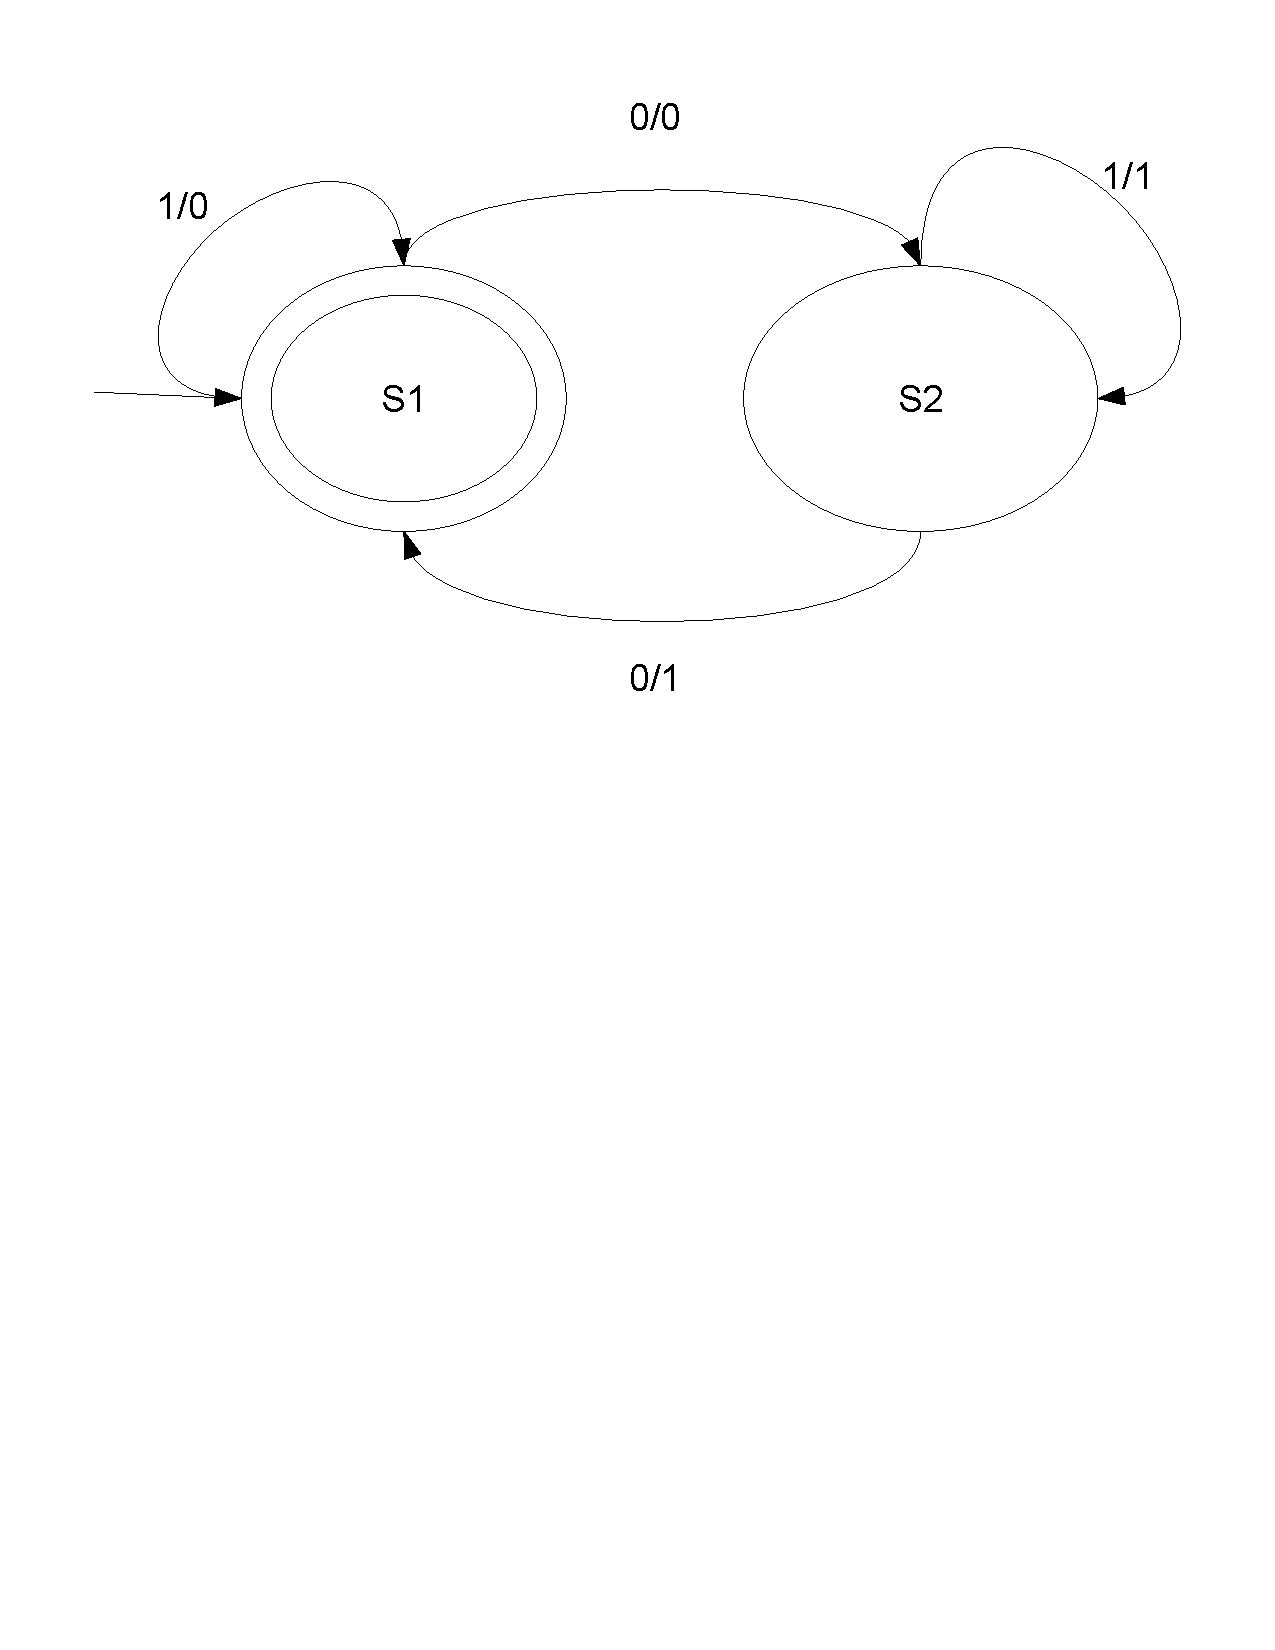
\includegraphics[trim= 15mm 150mm 15mm 10mm, clip ,width=200pt]{./images/state_mealy.pdf}    
    \caption{Moore and Mealy State Machines}
    \label{fig:state_moore_mealy}
\end{figure}

There are several ways a starting state can be defined as seen in figure \ref{fig:state_moore_mealy}.
One such way is to draw a edge that has no state connected to its tail, this generally looks like an edge out of nowhere. In our system we choose to use the UML symbol where the start state edge has a solid dot connected to the tail as shown in figure \ref{fig:state_uml_light}.

%diagram for UML state machines
\begin{figure}[htp]
    \centering
    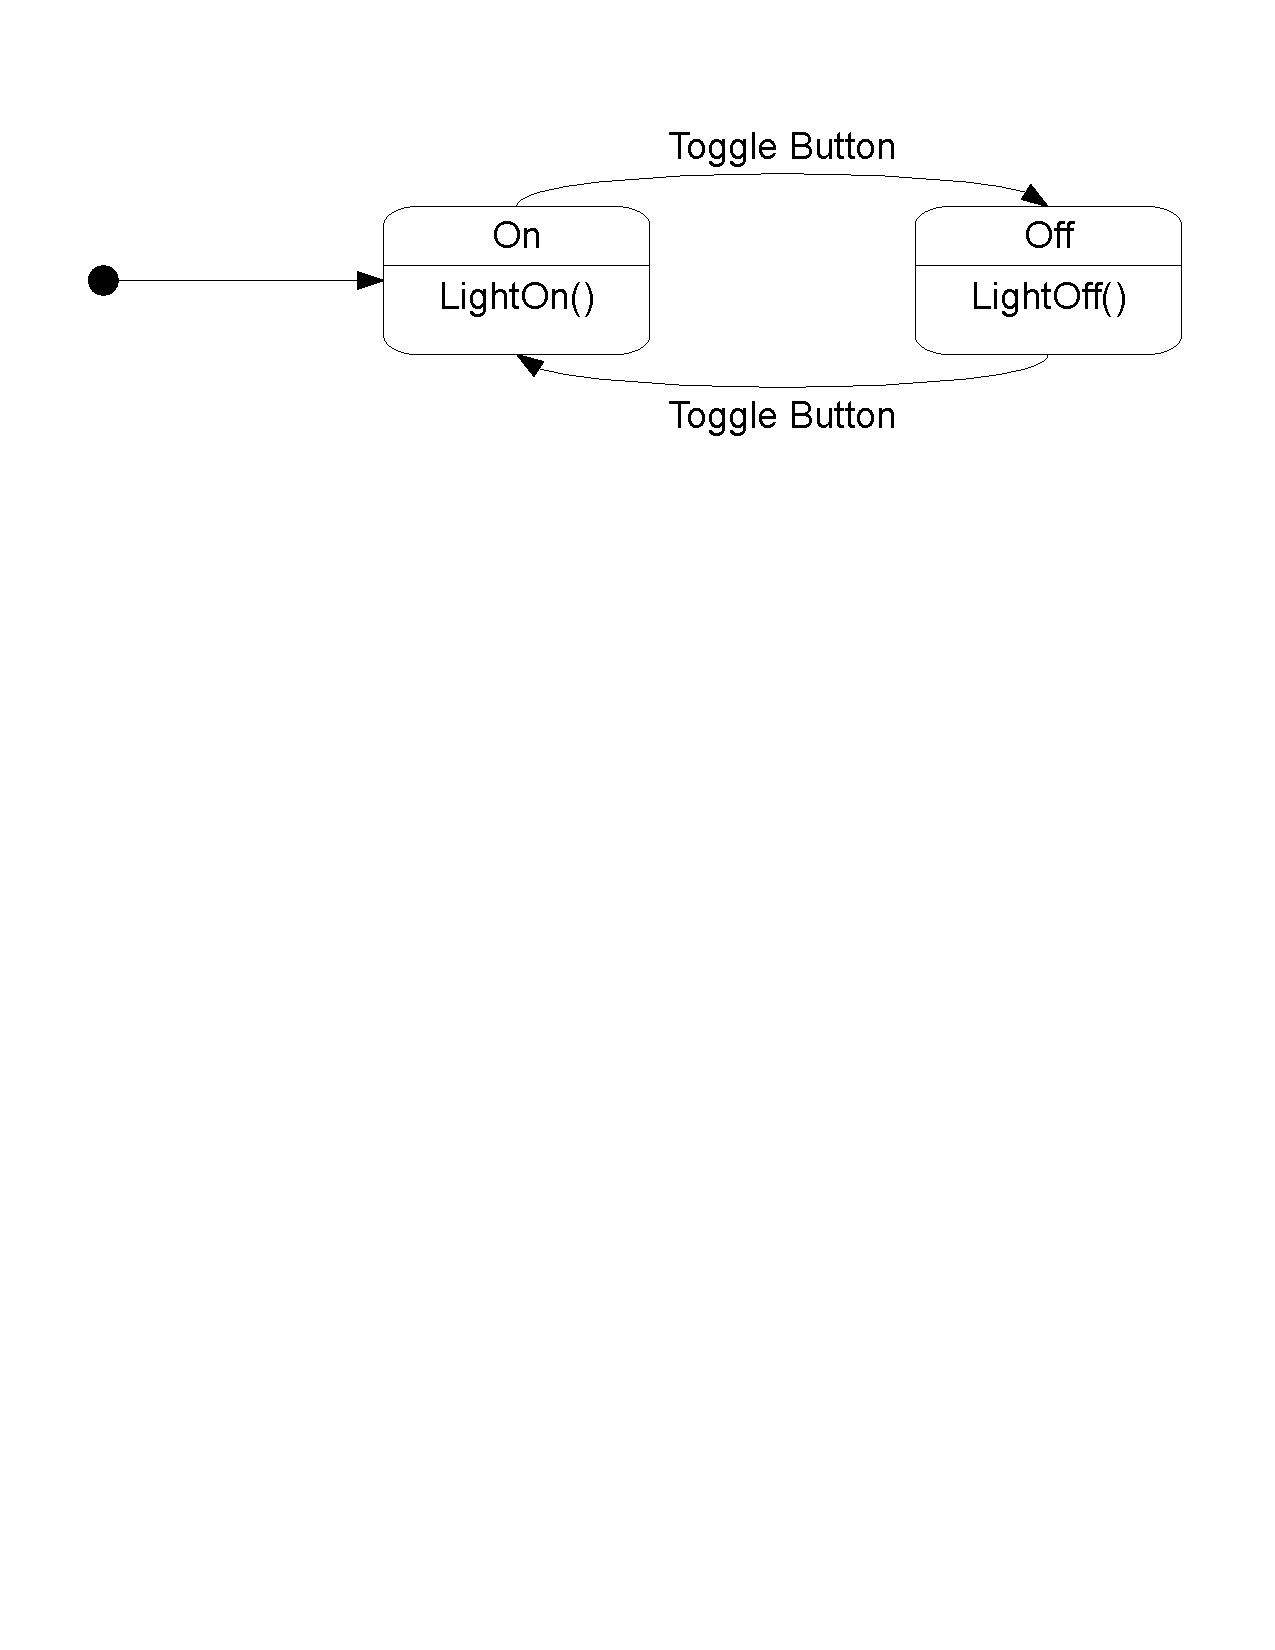
\includegraphics[trim= 15mm 200mm 15mm 10mm, clip ,width=\imgmedium]{./images/state_uml_light.pdf} 
    \caption{UML State Chart of a Togglable Light}
    \label{fig:state_uml_light}
\end{figure}

The accepting state is defined in state charts as any states where inputs are accepted. In other words this is generally a state in which the machine has successfully performed its task and is now ready to take on another one. Accepting states generally can reach all other states in the system. The symbol for an accepting state is a state with a double outline, this is shown in figure \ref{fig:state_moore_mealy}. For our implimentation we do not need to model this behavior and therefor the concept of accepting states have been left out for practical purposes.

The UML defined state charts as showin in figure \ref{fig:state_uml_light} also allow for state titles in each state which can be seen at the top of each state. In addition, each state may contain executed actions that will occur. In this case "LightOn()" and "LightOff()" refer to executed routines that are called once the "On" and "Off" states are reached respectively. The behavior is then once the state "On" is reached "LightOn()" is executed right away.

In a standard state chart a lot of implementation details can be hidden away and the diagram can be rather simple. In this example we see that there's no mention of how to turn on the light or turn off the light. Nor do we care if the light is connected to a particular port.

%Source wikipedia
TODO: The tyoe if state charts that we are using is a DIRECTED GRAPH with GUARDED EDGES. We have a starting state but not necessarily an ACCEPTING state.

TODO: Our state chart is very similar to an UML state diagram.

TODO: We might consider adapting our state chart to resemble UML digrams but that bit is under consideration. currently it does look very similar but edges do not have the correct formatting for guarded conditions on UML.

TODO: Minor detail, all of our states have an implicit edge going to END and will be used if no other conditions are true. We might consider showing the difference in the two.

TODO: Programming side, we need to enable saving because it's becoming a pain in the -bleep-.
